%%%%%%%%%%%%%%%%%%%%%%%%%%%%%%%%%%%%%%%%%%%%%%%%%
%%%
%%% Auteur : Stéphane Péchard - stephane.pechard@univ-nantes.fr
%%% Fichier : a-base.tex - annexe A : Élaboration d'une base de contenu et de séquences haute définition
%%% Version : 0.1
%%% Date : 2007/12/04
%%%
%%%%%%%%%%%%%%%%%%%%%%%%%%%%%%%%%%%%%%%%%%%%%%%%%

%%%%%%%%%%%%%%%%%%%%%%%%%%%%%%%%%%%%%%%%%%%%%%%%%
% citation
%%%%%%%%%%%%%%%%%%%%%%%%%%%%%%%%%%%%%%%%%%%%%%%%%
% \unecitation{6.5}{On ne connait pas complètement une science tant qu'on n'en sait pas l'histoire.}{Auguste Compte (1798 -- 1857)} ?? % FIXME citation
%%%%%%%%%%%%%%%%%%%%%%%%%%%%%%%%%%%%%%%%%%%%%%%%%
\chapter[Base de contenus et de séquences TVHD et notes subjectives de qualité]{Base de contenus et de séquences TVHD \\et notes subjectives de qualité} \label{annex:base}
\opt{final}{\lettrine[lines=4, loversize=-0.1, lraise=0.15]{Q}{ue ce soit pour l'évaluation}}\opt{nofinal}{Que ce soit pour l'évaluation} de la perception des dégradations ou pour l'évaluation des performances de critères objectifs de qualité vidéo, il est nécessaire de disposer d'une base de séquences vidéo set de notes subjectives de qualité associées. De plus, suivant la méthodologie d'évaluation utilisée, nous devons disposer de la version non dégradée et de différentes versions dégradées. VQEG possède déjà une telle base au format TVSD~\cite{vqeg-frtv1,vqeg-frtv2}, mais il n'en existe pas en TVHD. L'idéal serait que la communauté scientifique se dote d'une base commune~\cite{koh-vpqm2006} afin de pouvoir comparer les résultats issus des études de chacun.

Dans l'idéal, une telle base est constituée de trois éléments : les contenus non dégradés, pour chacun d'eux une ou plusieurs versions dégradées et les MOS \emph{Mean Opinion Score} correspondants. Chaque élément requiert une attention particulière. Tout d'abord, les contenus ne doivent pas avoir subi de dégradations, ce qui oblige à les obtenir directement des diffuseurs ou des producteurs. En effet, l'enregistrement après diffusion contient justement (du fait de la compression) des dégradations que nous cherchons à évaluer. Le fait de travailler sur des séquences haute définition rend l'obtention de tels contenus particulièrement délicate. Les productions actuelles en haute définition sont en effet soumises à droit d'auteurs, que les diffuseurs négocient avec les producteurs. Les contenus comme le sport ou les spectacles, particulièrement intéressants du fait de leur popularité, sont onéreux et non redistribuables. De plus, produire ses propres contenus au format haute définition demande du temps et des compétences techniques qu'il est généralement difficile de rassembler à un cout raisonnable. C'est pourquoi la quantité de contenus haute définition disponibles dans la communauté scientifique est faible et la constitution d'une base commune toujours d'actualité.

Créer des versions dégradées de tels contenus requiert un système dégradant. Cela peut servir à en évaluer l'impact sur la perception des dégradations. Dans cette étude, nous nous sommes intéressés à un système dégradant de type codeur \avc. Pour un même contenu, nous effectuons plusieurs codages \avc, correspondant chacun à un taux de compression donné. Nous n'utilisons pas ici de dégradations synthétiques comme l'application artificielle de flou, d'effet de bloc ou de bruit. Ainsi, le système dégradant est réaliste car il correspond aux dégradations produites par la compression de la TVHD en vue de sa diffusion.

Les notes subjectives de qualité sont la véritable valeur ajoutée majeure d'une telle base. Pour les obtenir, cela nécessite de disposer d'une infrastructure technique importante et d'avoir le savoir-faire de la réalisation de tests avec observateurs et de l'exploitation des données brutes. Le chapitre~\ref{chap:evalSubj} propose une description de l'obtention de ces notes subjectives.

Nous présentons ici les différents contenus utilisés pour la réalisation de nos campagnes de tests subjectifs et pour l'évaluation de nos critères objectifs de qualité vidéo. Regroupés selon leur provenance, ces contenus n'ont pas tous les mêmes caractéristiques. C'est pourquoi nous les détaillerons. Les points communs à tous ces contenus non dégradés sont leur résolution spatiale 1920\texttimes1080, leur mode entrelacé et leur cadence de 25 images par seconde (soit 50 trames par seconde). Les caractéristiques du codeur \avc{} utilisé et des séquences créées avec celui-ci seront détaillées. Enfin, nous donnerons les résultats obtenus lors des tests subjectifs.


\section{Contenus non dégradés}
Nous disposons d'une base de 24 contenus non dégradés. Cette base est assez hétérogène. En effet, elle est structurée en trois sous-ensembles, selon les provenances et les caractéristiques techniques des fichiers informatiques. Le premier sous-ensemble contient les seuls contenus non libres de droit de la base. Il provient de la chaine belge de télévision haute définition Euro1080. Les deux autres ensembles proviennent du même fournisseur, la chaine de télévision suédoise SVT \emph{(Sveriges Television)}. Cependant, ces deux derniers ensembles présentent quelques différences.


\subsection{Sous-base Euro1080} \label{ssec:seq-euro1080}
Cette première sous-base est constituée de huit contenus non libres de droit, donc uniquement utilisables dans un but scientifique, sans pouvoir être redistribués. Deux sous-ensembles se détachent, suivant la durée. Le premier est formé de contenus de douze secondes de durée, soit 300 images. Il est nommé Euro1080-1 et contient les contenus nommés \emph{Concert}, \emph{Foot}, \emph{Movie} et \emph{Voile}. Le second est formé de contenus de neuf secondes de durée, soit 225 images. Il est nommé Euro1080-2 et contient les contenus nommés \emph{Crédits}, \emph{Golf}, \emph{Show} et \emph{Standing}. Tous sont au format 4$:$2$:$2. Notons également que certains de ces contenus possèdent des changements de plan. Il s'agit de \emph{Foot}, \emph{Voile}, \emph{Crédits} et \emph{Show}, qui contiennent respectivement un, quatre, trois et un changement de plan. La figure~\ref{fig:sequencesC} présente une image issue de chacun de ces contenus, accompagnée d'une courte description. Les huit contenus forment une sous-base nommée Euro1080.

\begin{figure}[htbp]
  \centering
  \subfloat[\emph{Concert} : en intérieur, faible luminance]{\includegraphics[width=0.24\linewidth]{img/sequences/concert}}\hfill
  \subfloat[\emph{Foot} : en extérieur, traveling horizontal puis plan sur les joueurs]{\includegraphics[width=0.24\linewidth]{img/sequences/foot}}\hfill
  \subfloat[\emph{Movie} : en intérieur, traveling et zoom, peu de mouvement]{\includegraphics[width=0.24\linewidth]{img/sequences/movie}}\hfill
  \subfloat[\emph{Voile} : en extérieur, plusieurs plans sur des bateaux en mer]{\includegraphics[width=0.24\linewidth]{img/sequences/voile}}\\
  \subfloat[\emph{Crédits} : en intérieur, faible luminance, défilement de texte, plusieurs plans]{\includegraphics[width=0.24\linewidth]{img/sequences/credits}}\hfill
  \subfloat[\emph{Golf} : en extérieur, faible mouvement]{\includegraphics[width=0.24\linewidth]{img/sequences/golf}}\hfill
  \subfloat[\emph{Show} : en intérieur, zoom puis plan fixe]{\includegraphics[width=0.24\linewidth]{img/sequences/show}}\hfill
  \subfloat[\emph{Standing} : en intérieur, plan fixe sur orateur, très faible mouvement]{\includegraphics[width=0.24\linewidth]{img/sequences/standing}}\\
  \caption{Illustration des contenus de la sous-base Euro1080.}
  \label{fig:sequencesC}
\end{figure}


\subsection{Sous-base SVT2002} \label{ssec:seq-svt}
Quatre contenus au format PAL ont été réalisés par la chaine de télévision suédoise SVT en 2002. Librement mis à la disposition de la communauté scientifique, ils ont été spécifiquement tournés pour la recherche scientifique~\cite{svt-assesstudy}. L'un des buts avoués de leur réalisation est la mise en défaut des codeurs. Cela explique la complexité des contenus, non représentative de la production classique en télévision. Notamment, le contenu \emph{Parkrun} est particulièrement difficile à coder.

Ces contenus ont tous une durée de 10 secondes, soit 250 images. Ce sont les seuls de notre base à être au format 4$:$2$:$0. La figure~\ref{fig:sequencesB} présente une image issue de chacun de ces contenus, accompagnée d'une courte description. Cette sous-base est nommée SVT2002.

\begin{figure}[htbp]
  \centering
  \subfloat[\emph{New Mobile \& Calendar} : en intérieur, mouvement lent]{\includegraphics[width=0.24\linewidth]{img/sequences/mobile}}\hfill
  \subfloat[\emph{Park Run} : en extérieur, traveling horizontal]{\includegraphics[width=0.24\linewidth]{img/sequences/parkrun}}\hfill
  \subfloat[\emph{Knightshields} : en intérieur, traveling et zoom]{\includegraphics[width=0.24\linewidth]{img/sequences/shields}}\hfill
  \subfloat[\emph{Stockholm Pan} : en extérieur, panorama, faible mouvement]{\includegraphics[width=0.24\linewidth]{img/sequences/stockholm}}\\
  \caption{Illustration des contenus de la sous-base SVT2002.}
  \label{fig:sequencesB}
\end{figure}


\subsection{Sous-base SVT2006} \label{ssec:seq-svt2006}
Douze contenus au format 65 mm nous ont également été fournis par la chaine de télévision suédoise SVT. Issus du même esprit d'ouverture que les contenus précédents, ils ont aussi été spécifiquement tournés en 2004 pour la recherche scientifique. Ils sont tous tirés d'un long contenu de six minutes, filmé au format 3840\texttimes2160 en mode progressif à 50 images par seconde. Cette version est ensuite déclinée à différentes résolutions inférieures, dont la haute définition 1920\texttimes1080 entrelacée. Tous les contenus ont une durée de 10 secondes, soit 250 images. Nous avons nous-mêmes procédé au découpage des séquences au sein de la vidéo originale, qui ne correspond donc pas à celui proposé par SVT. Pour ne pas confondre nos séquences avec celles issues du découpage du SVT, leurs noms sont différents. L'équipe de production a accompagné son travail d'une notice technique. Nous connaissons donc particulièrement bien les conditions de réalisation et le format des fichiers informatiques générés.

Les contenus sont tous au format 4$:$2$:$2 et le codage est de 10 bits par composante. La figure~\ref{fig:sequencesD} présente une image issue de chacun de ces contenus, accompagnée d'une courte description. Tous ces contenus ont été tournés en extérieur. Cette sous-base est nommée SVT2006.

\begin{figure}[htbp]
  \centering
  \subfloat[\emph{Above Marathon} : plan fixe sur une foule en mouvement rapide]{\includegraphics[width=0.24\linewidth]{img/sequences/above_marathon_250}}\hfill
  \subfloat[\emph{Captain} : gros plan sur un homme, chute d'eau en arrière-plan]{\includegraphics[width=0.24\linewidth]{img/sequences/captain_250}}\hfill
  \subfloat[\emph{Dance in the Woods} : plusieurs personnages en mouvement, fondu en entrée de séquence]{\includegraphics[width=0.24\linewidth]{img/sequences/dance_in_the_woods_250}}\hfill
  \subfloat[\emph{Duck Fly} : canards sur une étendue d'eau, puis envol]{\includegraphics[width=0.24\linewidth]{img/sequences/duck_fly_250}}\\
  \subfloat[\emph{Fountain Man} : plan fixe, chute d'eau en avant-plan]{\includegraphics[width=0.24\linewidth]{img/sequences/fountain_man_250}}\hfill
  \subfloat[\emph{Group Disorder} : mouvement latéral lent, passage chaotique de personnages]{\includegraphics[width=0.24\linewidth]{img/sequences/group_disorder_250}}\hfill
  \subfloat[\emph{Inside Marathon} : plan fixe, très fort mouvement dû au passage de coureurs en avant-plan]{\includegraphics[width=0.24\linewidth]{img/sequences/inside_marathon_250}}\hfill
  \subfloat[\emph{New Parkrun} :  mouvement latéral lent, personnages en mouvement]{\includegraphics[width=0.24\linewidth]{img/sequences/new_parkrun_250}}\\
  \subfloat[\emph{Rendezvous} : traveling horizontal lent]{\includegraphics[width=0.24\linewidth]{img/sequences/rendezvous_250}}\hfill
  \subfloat[\emph{Stockholm Travel} : survol d'une ville puis orientation vers les nuages, faible mouvement]{\includegraphics[width=0.24\linewidth]{img/sequences/stockholm_travel_250}}\hfill
  \subfloat[\emph{Tree Pan} : traveling vertical, très faible mouvement]{\includegraphics[width=0.24\linewidth]{img/sequences/tree_pan_250}}\hfill
  \subfloat[\emph{Ulriksdals} : survol puis zoom sur des arbres]{\includegraphics[width=0.24\linewidth]{img/sequences/ulriksdals_250}}\\
  \caption{Illustration des contenus de la sous-base SVT2006.}
  \label{fig:sequencesD}
\end{figure}


\subsection{Conclusion}
Nous venons de détailler les caractéristiques des différents contenus TVHD dont nous disposons. Le tableau~\ref{tab:baseContenus} récapitule les principales différences entre les trois sous-bases de contenus.

\begin{table}[htbp]
\centering
\begin{tabular}{ccccc}\toprule
\textbf{Sous-ensemble}	& \textbf{Nombre de contenus}	& \textbf{Format}	& \textbf{Nombre d'images} 	& \textbf{Droits}	\\\toprule
Euro1080-1 						& 4 												& 4$:$2$:$2 			& 300 										& non libres\\\midrule
Euro1080-2						& 4 												& 4$:$2$:$2 			& 225 										& non libres\\\midrule
SVT2002							& 4 												& 4$:$2$:$0 			& 250 										& libres\\\midrule
SVT2006							& 12 											& 4$:$2$:$2 			& 250 										& libres \\\bottomrule
\end{tabular}
\caption{Tableau récapitulatif des caractéristiques de la base de contenus à notre disposition.}
\label{tab:baseContenus}
\end{table}


\section{Génération de séquences dégradées}
Tous les contenus que nous venons de présenter ont été dégradés par le codeur de référence \avc~\cite{h264-jm}. Le profil principal \emph{(main profile)} et le niveau 4.0 \emph{(level 4.0)} sont utilisés pour coder les quatre contenus SVT2002. Les autres contenus sont codés en utilisant le profil étendu \emph{(high profile)} car le profil principal ne gère pas le 4$:$2$:$2 et le niveau 4.0.

Nous avons remarqué que le codeur avait besoin de coder quelques images pour stabiliser le fonctionnement du régulateur de débit. C'est pourquoi nous avons rajouté des images au début de chaque contenu avant de les coder. Afin de ne pas créer de discontinuité dans l'estimation du mouvement, ces images ont été ajoutées dans le sens inverse de leur apparition dans la séquence comme le montre la figure~\ref{fig:inversionImages}. De plus, les contenus étant entrelacés, les deux trames ont été inversées. Cette partie n'étant pas évalué, cela n'a pas d'influence. Pour les contenus SVT2002, 24 images, ont été ajoutées, soit presque une seconde. Pour les contenus Euro1080 et SVT2004, nous en avons ajouté 48, soit deux secondes environ.

\begin{figure}[htbp]
	\centering
	% schéma sur l'explication du codage H.264
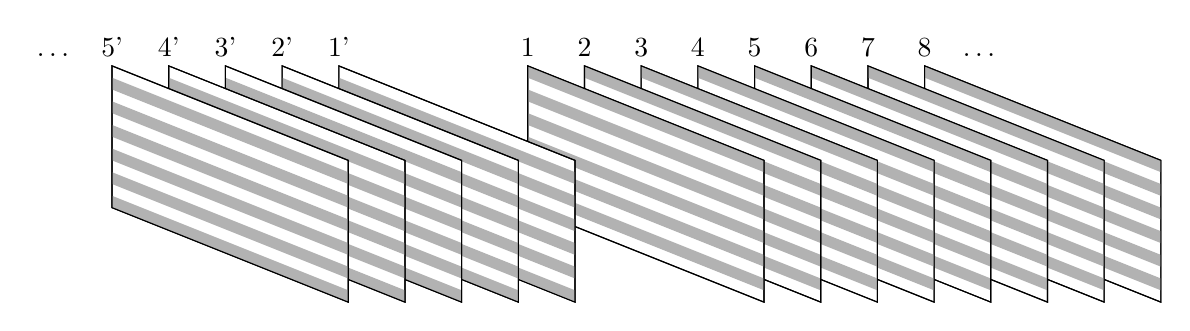
\begin{tikzpicture}[scale=0.6]
% en avant
\draw[fill=white] (18.4,0)--(23.4,-2)--(23.4,-5)--(18.4,-3) -- cycle;
\fill[fill=black!30] \foreach \i in {0,-0.5,-1,-1.5,-2,-2.5} {(18.4,-0.25+\i)--(23.4,-2.25+\i)--(23.4,-2+\i)--(18.4,\i) -- cycle};
\draw (18.4,0)--(23.4,-2)--(23.4,-5)--(18.4,-3) -- cycle;

\draw[fill=white] (17.2,0)--(22.2,-2)--(22.2,-5)--(17.2,-3) -- cycle;
\fill[fill=black!30] \foreach \i in {0,-0.5,-1,-1.5,-2,-2.5} {(17.2,-0.25+\i)--(22.2,-2.25+\i)--(22.2,-2+\i)--(17.2,\i) -- cycle};
\draw (17.2,0)--(22.2,-2)--(22.2,-5)--(17.2,-3) -- cycle;

\draw[fill=white] (16,0)--(21,-2)--(21,-5)--(16,-3) -- cycle;
\fill[fill=black!30] \foreach \i in {0,-0.5,-1,-1.5,-2,-2.5} {(16,-0.25+\i)--(21,-2.25+\i)--(21,-2+\i)--(16,\i) -- cycle};
\draw (16,0)--(21,-2)--(21,-5)--(16,-3) -- cycle;

\filldraw[fill=white] (14.8,0)--(19.8,-2)--(19.8,-5)--(14.8,-3) -- cycle;
\fill[fill=black!30] \foreach \i in {0,-0.5,-1,-1.5,-2,-2.5} {(14.8,-0.25+\i)--(19.8,-2.25+\i)--(19.8,-2+\i)--(14.8,\i) -- cycle};
\draw (14.8,0)--(19.8,-2)--(19.8,-5)--(14.8,-3) -- cycle;

\filldraw[fill=white] (13.6,0)--(18.6,-2)--(18.6,-5)--(13.6,-3) -- cycle;
\fill[fill=black!30] \foreach \i in {0,-0.5,-1,-1.5,-2,-2.5} {(13.6,-0.25+\i)--(18.6,-2.25+\i)--(18.6,-2+\i)--(13.6,\i) -- cycle};
\draw (13.6,0)--(18.6,-2)--(18.6,-5)--(13.6,-3) -- cycle;

\filldraw[fill=white] (12.4,0)--(17.4,-2)--(17.4,-5)--(12.4,-3) -- cycle;
\fill[fill=black!30] \foreach \i in {0,-0.5,-1,-1.5,-2,-2.5} {(12.4,-0.25+\i)--(17.4,-2.25+\i)--(17.4,-2+\i)--(12.4,\i) -- cycle};
\draw (12.4,0)--(17.4,-2)--(17.4,-5)--(12.4,-3) -- cycle;

\filldraw[fill=white] (11.2,0)--(16.2,-2)--(16.2,-5)--(11.2,-3) -- cycle;
\fill[fill=black!30] \foreach \i in {0,-0.5,-1,-1.5,-2,-2.5} {(11.2,-0.25+\i)--(16.2,-2.25+\i)--(16.2,-2+\i)--(11.2,\i) -- cycle};
\draw (11.2,0)--(16.2,-2)--(16.2,-5)--(11.2,-3) -- cycle;

\filldraw[fill=white] (10,0)--(15,-2)--(15,-5)--(10,-3) -- cycle;
\fill[fill=black!30] \foreach \i in {0,-0.5,-1,-1.5,-2,-2.5} {(10,-0.25+\i)--(15,-2.25+\i)--(15,-2+\i)--(10,\i) -- cycle};
\draw (10,0)--(15,-2)--(15,-5)--(10,-3) -- cycle;

\path (10,0) node[above] {1}
(11.2,0) node[above] {2}
(12.4,0) node[above] {3}
(13.6,0) node[above] {4}
(14.8,0) node[above] {5}
(16,0) node[above] {6}
(17.2,0) node[above] {7}
(18.4,0) node[above] {8}
(19.6,0) node[above] {\dots};

% en arrière
\filldraw[fill=white] (6,0)--(11,-2)--(11,-5)--(6,-3) -- cycle;
\fill[fill=black!30] \foreach \i in {-0.25,-0.75,-1.25,-1.75,-2.25,-2.75} {(6,-0.25+\i)--(11,-2.25+\i)--(11,-2+\i)--(6,\i) -- cycle};
\draw (6,0)--(11,-2)--(11,-5)--(6,-3) -- cycle;

\filldraw[fill=white] (4.8,0)--(9.8,-2)--(9.8,-5)--(4.8,-3) -- cycle;
\fill[fill=black!30] \foreach \i in {-0.25,-0.75,-1.25,-1.75,-2.25,-2.75} {(4.8,-0.25+\i)--(9.8,-2.25+\i)--(9.8,-2+\i)--(4.8,\i) -- cycle};
\draw (4.8,0)--(9.8,-2)--(9.8,-5)--(4.8,-3) -- cycle;

\filldraw[fill=white] (3.6,0)--(8.6,-2)--(8.6,-5)--(3.6,-3) -- cycle;
\fill[fill=black!30] \foreach \i in {-0.25,-0.75,-1.25,-1.75,-2.25,-2.75} {(3.6,-0.25+\i)--(8.6,-2.25+\i)--(8.6,-2+\i)--(3.6,\i) -- cycle};
\draw (3.6,0)--(8.6,-2)--(8.6,-5)--(3.6,-3) -- cycle;

\filldraw[fill=white] (2.4,0)--(7.4,-2)--(7.4,-5)--(2.4,-3) -- cycle;
\fill[fill=black!30] \foreach \i in {-0.25,-0.75,-1.25,-1.75,-2.25,-2.75} {(2.4,-0.25+\i)--(7.4,-2.25+\i)--(7.4,-2+\i)--(2.4,\i) -- cycle};
\draw (2.4,0)--(7.4,-2)--(7.4,-5)--(2.4,-3) -- cycle;

\filldraw[fill=white] (1.2,0)--(6.2,-2)--(6.2,-5)--(1.2,-3) -- cycle;
\fill[fill=black!30] \foreach \i in {-0.25,-0.75,-1.25,-1.75,-2.25,-2.75} {(1.2,-0.25+\i)--(6.2,-2.25+\i)--(6.2,-2+\i)--(1.2,\i) -- cycle};
\draw (1.2,0)--(6.2,-2)--(6.2,-5)--(1.2,-3) -- cycle;

\path (6,0) node[above] {1'}
(4.8,0) node[above] {2'}
(3.6,0) node[above] {3'}
(2.4,0) node[above] {4'}
(1.2,0) node[above] {5'}
(0,0) node[above] {\dots};

\end{tikzpicture}

	\caption{Schéma de l'ajout d'images dans l'ordre temporel inverse avec inversion des trames.}
	\label{fig:inversionImages}
\end{figure}

Les paramètres de codage sont les suivants.

Nous utilisons un GOP \emph{(Group of picture)} de douze images et deux images bidirectionnelles B, ce qui donne la structure de GOP suivante :

\begin{center}
I B B P B B P B B P B B
\end{center}

Le fichier codé en sortie du codeur est un bitstream H.264 que nous n'utilisons pas directement. Il est d'abord décodé avec le codeur de référence, afin de générer un fichier informatique de même type que celui en entrée du codeur. C'est pourquoi nous ne nous sommes pas particulièrement intéressé à la configuration du codeur entropique.

Sept débits différents ont été produits par contenu, ce qui fait un ensemble de 168 séquences dégradées. Les débits utilisés, définis par un panel d'experts, sont présentés en Mbps dans le tableau~\ref{tab:bitratesHD}. Les gammes de débits peuvent être très différentes d'un contenu à un autre. Ceci est dû aux différences de complexité spatio-temporelle des contenus. Pour chaque contenu, les gammes de débits conduisent à couvrir l'échelle catégorielle de qualité de \emph{mauvais} à \emph{excellent}.

\begin{table}[htbp]
\centering
\begin{tabular}{cc}\toprule
\textbf{contenu}				& \textbf{débits TVHD (Mbps)} \\ \toprule
\emph{New Mobile \& Calendar}	& 2,25 ; 2,5 ; 3,15 ; 4 ; 5 ; 7 ; 10 \\ \midrule
\emph{Parkrun}					& 8 ; 12 ; 16 ; 18 ; 20 ; 24 ; 28 \\ \midrule
\emph{Knightshields}			& 2,25 ; 3 ; 4 ; 5 ; 6 ; 7 ; 8 \\ \midrule
\emph{Stockholm Pan}			& 1,625 ; 1,875 ; 2,25 ; 3 ; 3,6 ; 4 ; 6 \\ \midrule
\emph{Concert}					& 4 ; 8 ; 10 ; 14 ; 18 ; 24 ; 30 \\ \midrule
\emph{Foot}						& 4 ; 6 ; 10 ; 14 ; 18 ; 22 ; 26 \\ \midrule
\emph{Movie}					& 2,5 ; 4 ; 7 ; 8 ; 9 ; 10 ; 14 \\ \midrule
\emph{Voile}					& 2,5 ; 4 ; 6 ; 8 ; 9 ; 11 ; 12 \\ \midrule
\emph{Crédits}					& 4 ; 6 ; 7 ; 8 ; 9 ; 10 ; 14 \\ \midrule
\emph{Golf}						& 1 ; 1,5 ; 2 ; 2,5 ; 3 ; 4 ; 6 \\ \midrule
\emph{Show}						& 2 ; 3 ; 4 ; 8 ; 10 ; 14 ; 22 \\ \midrule
\emph{Standing}					& 0,75 ; 1,25 ; 2 ; 3 ; 5 ; 6 ; 8 \\ \midrule
\emph{Above Marathon}			& 5 ; 8 ; 10 ; 12 ; 16 ; 24 ; 32 \\ \midrule
\emph{Captain}					& 1 ; 3 ; 5 ; 6 ; 8 ; 12 ; 18 \\ \midrule
\emph{Dance in the Woods}		& 3 ; 5 ; 6 ; 8 ; 10 ; 14 ; 18 \\ \midrule
\emph{Duck Fly}					& 4 ; 6 ; 8 ; 12 ; 16 ; 20 ; 32 \\ \midrule
\emph{Fountain Man}				& 1 ; 2 ; 5 ; 8 ; 9 ; 12 ; 20 \\ \midrule
\emph{Group Disorder}			& 2 ; 4 ; 7 ; 8 ; 12 ; 16 ; 20 \\ \midrule
\emph{Inside Marathon}			& 3 ; 4 ; 6 ; 8 ; 10 ; 14 ; 16 \\ \midrule
\emph{New Parkrun}				& 2 ; 4 ; 6 ; 8 ; 10 ; 14 ; 20 \\ \midrule
\emph{Rendezvous}				& 4 ; 6 ; 8 ; 10 ; 14 ; 18 ; 24 \\ \midrule
\emph{Stockholm Travel}			& 1 ; 4 ; 6 ; 8 ; 10 ; 16 ; 20 \\ \midrule
\emph{Tree Pan}					& 1,25 ; 1,5 ; 2 ; 2,5 ; 3 ; 5 ; 8 \\ \midrule
\emph{Ulriksdals}				& 1 ; 2 ; 4 ; 6 ; 8 ; 12 ; 16 \\ \bottomrule
\end{tabular}
\caption{Débits de compression utilisés avec le codeur de référence \avc{}. Ils ont été sélectionnés par des experts pour chaque séquence HD.}
\label{tab:bitratesHD}
\end{table}


\section{Évaluation subjective de la qualité des séquences dégradées par le codeur de référence \avc}
Cette évaluation permet de caractériser le codeur de référence~\cite{h264-jm} en termes de qualité visuelle en fonction du débit pour chacun des contenus. La réduction du débit lié à la quantification après transformation et compensation de mouvement se transforme en dégradations perçues par l'observateur. Suivant le débit, la qualité ressentie est alors équivalente, inférieure ou très inférieure à celle de la référence. C'est une valeur numérique représentant cette sensation que nous obtenons ici. Nous commençons par détailler les conditions dans lesquelles les tests ont été réalisés. Puis, les fonctions MOS--débit obtenus sont présentées et commentées.


\subsection{Conditions de test}
Le protocole utilisé est la méthode SAMVIQ~\cite{ebu-samviq} présentée section~\ref{tests:samviq}. L'écran de visualisation est de type LCD Philips T370HW01 d'une hauteur de 46 centimètres. Les 192 séquences de la section précédente sont présentées aux observateurs contenu par contenu. Ainsi, les tests sont effectués en six sessions de quatre contenus, soit 36 séquences. En effet, une session SAMVIQ est composée de neuf séquences, les sept traitements et les références explicite et cachée. Les observateurs ne sont pas systématiquement les mêmes d'une session à l'autre. Le tableau~\ref{tab:nbObsPerfCodeurRef} présente le nombre d'observateurs retenus pour chacune des sessions. La session SVT2006-1 contient les contenus \emph{Fountain Man}, \emph{Group Disorder}, \emph{Rendezvous} et \emph{Ulriksdals} ; la session SVT2006-2 les contenus \emph{Above Marathon}, \emph{Captain}, \emph{Dance in the Wood} et \emph{Duck Fly} ; la session SVT2006-3 les contenus \emph{Inside Marathon}, \emph{New Parkrun}, \emph{Stockholm Travel} et \emph{Tree Pan}.

\begin{table}[htbp]
\centering
\begin{tabular}[c]{m{2.5cm}cccccc}\toprule
\multirow{2}{2.5cm}{\strong{session}} & \multirow{2}{1.5cm}{SVT2002} & \multicolumn{2}{c}{Euro1080} & \multicolumn{3}{c}{SVT2006}\\  \cmidrule(r){3-7}
				& 	& 1 	& 2 	& 1 	& 2 	& 3\\ \midrule
\centering\strong{nombre d'observateurs} & 22		& 21					& 22					& 16					& 15					& 19\\ \bottomrule
\end{tabular}
\caption{Nombre d'observateurs retenus après rejet pour chacune des sessions de l'évaluation subjective des séquences dégradées par le codeur de référence \avc.}
\label{tab:nbObsPerfCodeurRef}
\end{table}


\subsection{Résultats des tests subjectifs}
La figure~\ref{fig:MOSrateCodeurRefHD} présente les MOS et leurs intervalles de confiance à 95\% en fonction du débit pour les 24 contenus codés à sept débits chacun. Comme il est prévisible, la qualité subjective augmente globalement avec le débit. Cependant, il arrive que la courbe ne soit pas monotone croissante. En effet, le codeur de référence n'est pas réputé pour posséder une régulation débit-distorsions très efficace. Nos contacts avec des spécialistes de ce codeur confirment cette conclusion.

Les intervalles de confiance à 95\% obtenus sur l'ensemble des évaluations sont de mesure comprise entre 2,753 et 11,514, avec une moyenne de 6,906. Leur histogramme est présenté sur la figure~\ref{fig:histoIC}. Les faibles valeurs obtenues montre la bonne précision que permet le protocole SAMVIQ, avec un nombre restreint d'observateurs.

\begin{figure}[htbp]
\centering
\begin{tikzpicture}[xscale=0.5, yscale=0.05]
	\draw[ycomb, black,line width=6pt] plot[] file {plot/data/08-histoIC.txt};
	\path (1,0) node {0} (1,15) node {15} (1,31) node {31} (1,48) node {48} (2,-4) node {2} (3,-4) node {3} (4,-4) node {4} (5,-4) node {5} (6,-4) node {6} (7,-4) node {7} (8,-4) node {8} (9,-4) node {9} (10,-4) node {10} (11,-4) node {11};
\end{tikzpicture}
\caption{Histogramme des intervalles de confiance à 95\% obtenus sur l'ensemble des évaluations subjective effectuées sur la base de séquences codées.}
\label{fig:histoIC}
\end{figure}

Enfin, la dépendance au contenu est ici évidente, avec des qualités équivalentes pour des débits très différents, comme par exemple entre les contenus \emph{Parkrun} et \emph{Tree Pan}. \emph{Parkrun} a un MOS de 26,32 à 8 Mbps et de 69,09 à 28 Mbps, alors que \emph{Tree Pan} obtient 22,125 à 1,25 Mbps et 70,875 à 8 Mbps.

\begin{figure}[htbp]
\centering
\subfloat{\includegraphics[page=1, width=0.48\linewidth, trim= 70 50 90 70]{plot/debit-mosHD.pdf}}\hfill
\subfloat{\includegraphics[page=2, width=0.48\linewidth, trim= 70 50 90 70]{plot/debit-mosHD.pdf}}\\
\subfloat{\includegraphics[page=3, width=0.48\linewidth, trim= 70 50 90 70]{plot/debit-mosHD.pdf}}\hfill
\subfloat{\includegraphics[page=4, width=0.48\linewidth, trim= 70 50 90 70]{plot/debit-mosHD.pdf}}\\
\subfloat{\includegraphics[page=5, width=0.48\linewidth, trim= 70 50 90 70]{plot/debit-mosHD.pdf}}\hfill
\subfloat{\includegraphics[page=6, width=0.48\linewidth, trim= 70 50 90 70]{plot/debit-mosHD.pdf}}\\
\caption{Notes de qualité en fonction du débit, exprimé en Mbps, obtenues pour le codeur de référence \avc{} par les séquences de TVHD.}
\label{fig:MOSrateCodeurRefHD}
\end{figure}


\section{Conclusion}
Cette annexe a présenté les éléments de la base de contenus et de séquences que nous avons constituée lors de plusieurs campagnes de tests subjectifs. Trois parties distinctes ont été détaillées :  les contenus originaux non dégradées, les séquences compressées par le codeur de référence \avc{} et enfin les notes de qualité associées à chacune des séquences originales ou codées produites. Au total, 24 contenus ont été codés à sept débits différents. Cette base est donc constituée de 192 séquences. Cependant, il convient de noter que parmi cet ensemble, huit contenus ne sont pas libres de droit. Nous ne pourrons donc pas en faire bénéficier la communauté scientifique.


\ornementChapitre
